% ADvoice manuscript draft for npj Digital Medicine
% Revised on 2026-09-24. Historical evaluation results are retained as a
% locked snapshot; the redesigned Agent pilot is reported only after gate review.
% The Springer Nature sn-jnl class is used for internal authoring only.
% npj Digital Medicine does not require this class at initial submission.

\documentclass[pdflatex,sn-nature]{sn-jnl}

\usepackage{graphicx}
\usepackage{booktabs}
\usepackage{amsmath}
\usepackage{tabularx}
\usepackage{threeparttable}
\usepackage{xcolor}

\raggedbottom

\begin{document}

\title[Evidence-governed speech screening]{Evidence-governed cognitive-state fusion for task-aware speech screening}

\author*[1]{\fnm{AUTHOR} \sur{INPUT REQUIRED}}\email{AUTHOR.INPUT@REQUIRED}
\affil*[1]{\orgdiv{Department}, \orgname{Institution}, \orgaddress{\city{City}, \country{Country}}}

\abstract{Speech-based cognitive screening is scalable, but models trained across heterogeneous tasks and languages can mistake task structure or recording quality for disease evidence. We developed an evidence-governed framework that links source segments to MetricEvidence objects, task-conditioned cognitive StateCards, supervised predictions and a bounded diagnostic Agent. The redesigned Agent is evaluated as an independent evidence reader and limited state-revision mechanism rather than as a narrator of a frozen probability. Five prespecified arms separate base calibration, Agent judgment and state replay. The locked historical evaluation included ten retrospective datasets and 745 held-out analysis units; it showed broad cross-task feasibility but remained below SpeechCARE on PREPARE and did not demonstrate Agent-mediated predictive gain. The new pilot therefore requires complete out-of-fold provenance, matched-row baselines, class-specific benefit--harm accounting, failure and cost denominators, and an independent release gate before any superiority claim. This design treats traceability as a computational constraint on prediction rather than post-hoc explanatory text.}

\keywords{cognitive impairment, speech, evidence governance, clinical decision support, multimodal learning, large language model}

\maketitle

\section{Introduction}\label{sec:introduction}

Cognitive impairment is often identified only after functional difficulties have become clinically apparent, whereas specialist assessment, neuroimaging and fluid biomarkers are difficult to deploy as population-scale first-line tests \cite{Xue2024,Verghese2024}. Speech can be collected repeatedly and remotely, and it reflects performance across language, executive, memory and processing-speed domains rather than a single disease-specific lesion \cite{Heitz2026}. This distinction defines the intended use of speech artificial intelligence: it may identify people whose cognitive performance warrants further assessment, but speech alone cannot establish Alzheimer pathology, determine aetiology or replace formal clinical evaluation. The clinically relevant target is therefore cognitive-risk screening and referral support with explicit uncertainty and evidence sufficiency.

Speech-based models have progressed from hand-crafted acoustic and linguistic variables to multilingual pretrained representations and adaptive multimodal fusion. SpeechCARE combines acoustic, linguistic and demographic representations with a learned gating network across languages and speech tasks \cite{Azadmaleki2025}. Such systems can learn whether a case is better represented by audio or text, but a modality weight does not identify which cognitive function was observable, which patient behaviour was abnormal, or whether the apparent signal arose from an interviewer, task duration, automatic speech recognition (ASR) error or recording device. A recent systematic review similarly found persistent gaps in stakeholder evaluation, real-world validation and standardized assessment of explanations in speech-based cognitive models \cite{Shankar2025}. Predictive discrimination and post-hoc attribution therefore do not by themselves provide a patient-level clinical evidence chain.

A parallel literature has integrated prediction and language-model reasoning in cognitive decision support. Multimodal systems using clinical, cognitive and imaging data have supported differential dementia assessment and clinician decision making \cite{Qiu2022,Xue2024}. The Multimodal Evidence-Driven Reasoning Framework (MEDRF) combined a hierarchical classifier with retrieval of analogous cases and medical literature, improving three-class external accuracy from 0.706 to 0.753 and producing physician-rated reports \cite{Hu2026}. Agentic systems have also operated over longitudinal clinical notes to predict Alzheimer disease or detect documented cognitive concerns \cite{Li2025,Tian2026}. These studies establish the value of combining statistical prediction and language-model reasoning, but they do not solve the measurement problems specific to speech: task-dependent observability, speaker-role separation, recording reliability, confounding, segment-level provenance and permission to translate a low-level feature into a clinician-facing statement.

Here we investigate whether evidence-governed cognitive states can serve as a common interface between heterogeneous speech tasks, supervised prediction and clinical reporting. The framework routes each recording by task, language, modality and speaker role; converts each measurement into a MetricEvidence object; estimates task-conditioned StateCards against training-fold reference participants; and fits a matched supervised base from complete out-of-fold predictions. A single diagnostic Agent then reads a label-blind package that omits the base probability, cites eligible evidence, and may request a bounded remeasurement or state revision. A deterministic executor applies accepted operations and recomputes affected states. Five prespecified arms---raw base, calibrated base, base plus Agent judgment, base plus state replay, and their joint model---separate calibration from Agent and replay contributions. Evaluation separates medical prediction from evidence integrity, traceability, class-specific harm, fallback and computational cost.

\section{Related work and positioning}\label{sec:related}

\subsection{Speech-based cognitive screening}

Speech research in cognitive impairment has developed along three technical lines. Early systems relied on hand-crafted acoustic and linguistic variables, including pause timing, speaking rate, lexical diversity, syntactic complexity and semantic content. More recent systems use pretrained speech and language encoders to learn representations that are less dependent on a manually selected feature inventory. A third line combines modalities or tasks through attention, late fusion or learned gates. Across these approaches, speech is best understood as a proxy for performance in several cognitive domains rather than a direct assay of Alzheimer pathology \cite{Heitz2026}. The distinction is clinically important: a model can support low-burden risk screening while remaining unable to establish disease aetiology.

SpeechCARE is the closest predictive benchmark to the present work \cite{Azadmaleki2025}. It combines multilingual HuBERT audio representations, multilingual text embeddings and age information, and learns sample-specific modality weights through adaptive gating. Its PREPARE evaluation demonstrates that multilingual and multi-task speech can be integrated without a separate model for every task. However, modality-level weights answer which representation the classifier used, not whether a cognitive state was observable under the current task, which patient behaviour supplied the evidence, or whether the signal was contaminated by interviewer structure, ASR quality, duration or device characteristics. Our work treats those measurement and provenance questions as part of the model interface rather than as post-hoc explanation.

Explainable speech systems have used feature attribution, attention visualization, saliency and natural-language summaries. A recent systematic review found that explanation methods were rarely assessed with patients or clinicians and that real-world validation remained limited \cite{Shankar2025}. Low-level attribution is also vulnerable to overinterpretation: a spectral coefficient or encoder dimension may aid classification without constituting a clinically reportable mechanism. This motivates our explicit separation among clinical evidence, model-only auxiliary information and quality control.

\subsection{Multimodal cognitive decision support}

Clinical decision-support studies have combined neuropsychological tests, demographics, structural imaging and electronic health records to classify cognitive stage or dementia aetiology \cite{Qiu2022,Xue2024}. These systems address a different point in the care pathway from speech screening. They operate after richer clinical information has been collected and can use variables with stronger diagnostic specificity. Their principal methodological challenge is integrating heterogeneous clinical evidence and missing modalities, whereas speech screening must additionally determine whether the elicitation task made a particular behaviour measurable.

MEDRF represents the closest evidence-driven clinical framework \cite{Hu2026}. It couples a hierarchical classifier with retrieval of similar cases and medical literature, allowing a language model to refine ambiguous predictions and generate supporting explanations. MEDRF's hierarchy is diagnostic: cognitive status is followed by disease subtype and aetiology. Our hierarchy is a measurement hierarchy: source segments support metrics, metrics support cognitive states, and states support a screening estimate. The two approaches are therefore complementary. MEDRF demonstrates how retrieved clinical knowledge can support specialist reasoning; the present study asks how evidence should be constructed and governed before a language model is allowed to reason over speech.

\subsection{Agentic reasoning and the remaining gap}

Language-model agents have been used to synthesize longitudinal notes, retrieve relevant observations and detect documented cognitive concerns \cite{Li2025,Tian2026}. These systems show that an Agent can organize temporally distributed evidence and communicate a decision. They also expose a safety issue: fluent reasoning can cite unsupported facts, conflate a risk factor with an observed impairment or change a model prediction without a reproducible measurement basis. In speech, this risk is amplified because the input contains interviewer speech, task prompts, silence, recording artefacts and ASR errors.

The unresolved gap is therefore not simply multimodal fusion or report generation. It is the absence of a common, machine-verifiable evidence representation linking heterogeneous speech tasks to prediction and clinical communication. We address this gap with four design constraints. First, evidence is conditioned on task, language and speaker role. Second, every metric carries direction, reliability, missingness, confound and report-permission fields. Third, metrics are aggregated into observable cognitive StateCards with supporting and counterevidence. Fourth, the supervised model and diagnostic Agent operate over the same identifiers, and unsupported Agent proposals are rolled back. This positioning shifts the research question from whether an Agent can produce a plausible cognitive report to whether the complete decision can be reconstructed from permitted patient evidence.

\section{Methods}\label{sec:methods}

\subsection{Study design and intended use}

We conducted a retrospective, multi-dataset evaluation of speech-based cognitive-risk screening. The intended use was research screening and referral support. The system was not designed to establish Alzheimer pathology or replace clinical history, neurological examination, validated cognitive testing, imaging or biomarkers. The experimental unit was a participant, subject or public figure according to the source dataset. Repeated recordings from the same identity were aggregated or assigned to the same partition.

\subsection{Datasets and held-out partitions}

Ten locally available datasets were registered before the final aggregate evaluation: IAEAV, ADReSS 2020, ADReSSo 2021 diagnosis, ADReSSo 2021 progression, PROCESS-2, PREPARE, TAUKADIAL, DementiaBank Pitt, DementiaNet PublicFigures and NCMMSC 2021 AD. Source labels were retained rather than harmonized into a single clinical endpoint. Official subject-disjoint train--test partitions were used when labelled test data were available. Otherwise, deterministic stratified participant-disjoint holdouts of 20--30\% were created with a fixed project seed. All three conditions used identical held-out identities within each dataset.

For NCMMSC, only the distributed long-speech track was included; six-second clips and unlabelled recordings were excluded. For Pitt and other CHAT-derived data, patient and interviewer roles were parsed and only patient intervals were used for patient acoustic measurements. IAEAV patient segments were derived from distributed role annotations. For data without speaker roles, the limitation was recorded and role-dependent metrics were marked unavailable. Dataset-specific inclusion criteria and source licenses are provided in Supplementary Table~1. \textbf{[AUTHOR INPUT REQUIRED: insert ethics approvals, consent basis and exact data-use agreements.]}

\subsection{Audio, transcript and task preprocessing}

Audio was resampled to 16~kHz. Processing retained original duration and quality variables, including clipping, a signal-to-noise proxy and role coverage. Recordings were routed by language, task type, source channel and available speaker-role structure. Distributed transcripts were used when available; otherwise ASR used Whisper large-v3-turbo with automatic language selection. ASR outputs retained provenance and were assigned lower reliability when no human-verified transcript was available.

The deep acoustic pathway used a frozen multilingual HuBERT encoder (mHuBERT-147, pinned model revision). Up to 30~s per participant were split into 5~s windows with 25\% overlap. Window vectors were $L_2$ normalized, and participant-level mean and standard deviation vectors were supplied to a dense expert. A segment-attention expert was additionally eligible when sample size and audio coverage met prespecified thresholds. The deep text pathway used frozen multilingual-e5-base embeddings with a maximum input length of 512 tokens. These representations were model-only inputs and were not translated directly into disease mechanisms.

Hand-crafted measures covered pauses, voiced and non-voiced timing, speech-run continuity, rate, intensity, fundamental frequency, spectral descriptors, lexical specificity and diversity, utterance length, disfluency, repair and patient turn share. Availability depended on task, language, transcript quality and speaker roles. Spectral features and quality variables could aid prediction but were not reportable as clinical mechanisms.

Where source age metadata were available, age was encoded into prespecified fixed categories together with an explicit missing-age indicator. The categories were outcome-independent, were used only as optional model context and were never translated into patient-level cognitive evidence or a clinician-facing disease mechanism. Datasets without age metadata did not receive an imputed age category.

\subsection{MetricEvidence objects}

Each measured metric was stored as a MetricEvidence object containing the value, expected abnormal direction, training-reference median and scale, task scope, source modality, reliability, missingness, confound tags, evidence role, report permission and links to source segments. For metric $j$ in participant $i$, a fold-internal directional deviation was computed as

\begin{equation}
z_{ij}^{\mathrm{dir}} = d_j\frac{x_{ij}-\operatorname{median}_{\mathrm{CN,train}}(x_j)}{s_{j,\mathrm{CN,train}}},
\end{equation}

where $d_j\in\{-1,0,1\}$ encoded whether lower or higher values were expected to indicate greater impairment, and $s_j$ was a robust scale estimated only from reference participants in the current training fold. Near-constant or unavailable reference metrics were marked missing rather than divided by an arbitrarily small scale. Directional deviations were clipped to $[-5,5]$ before state aggregation to limit single-metric dominance.

Reliability was determined from design reliability and case-specific availability, transcript provenance, role coverage and quality flags. Quality-control variables had $d_j=0$ and could alter reliability or trigger a limitation but could not directly support a disease statement. This separation was enforced both in the model input schema and in report validation.

\subsection{Task-conditioned cognitive StateCards}

Metrics were mapped to prespecified cognitive or speech-behaviour states: pause and fluency burden, output efficiency, speech continuity, intensity stability, prosodic variation, low-level spectral pattern, lexical retrieval and specificity, lexical diversity, syntactic complexity, disfluency and repair, and interaction burden. Semantic coherence, information density and task performance were registered but disabled because validated multilingual scoring algorithms or task answer keys were not available.

For state $k$, the case score was the reliability-weighted mean of bounded directional metric deviations,

\begin{equation}
S_{ik}=\frac{\sum_{j\in\mathcal{M}_k} w_{jk}r_{ij}\,\operatorname{clip}(z_{ij}^{\mathrm{dir}},-5,5)}{\sum_{j\in\mathcal{M}_k} w_{jk}r_{ij}},
\end{equation}

where $w_{jk}$ was the prespecified within-state metric weight and $r_{ij}$ was participant-level reliability. The denominator also produced a state confidence estimate. StateCards stored severity, category, confidence, missing fraction, supporting metrics, counterevidence, task scope and local evidence segments. Overall states were retained for every case; task-specific states were added for multi-task recordings and selected only within training folds.

\subsection{Supervised task-conditioned fusion}

The supervised prediction pathway contained two small modules. Module A combined eligible experts representing clinical-language states, speech behaviour, auxiliary acoustics, interaction/task information, multilingual text embeddings, deep audio embeddings, segment trajectories and optional age context. Quality variables were used for reliability and ridge residualization rather than as a disease branch. Experts with cross-validated macro-AUROC below 0.52 were excluded. Auxiliary-acoustic influence was capped.

Fusion candidates included multinomial logistic stacking of expert log probabilities and reliabilities and a dynamic reliability gate with a 48-dimensional hidden layer. Selection used nested stratified cross-validation within the training data, with macro-F1 as the primary criterion and macro-AUROC as the tie-breaker. All branch models generated out-of-fold probabilities before the meta-model was fitted. Module B used cross-fitted evidence coverage, evidence reliability, confound burden, state-to-class prototype differences and Module A probabilities to learn a bounded residual correction. Blend strength, class offsets and temperature were selected in inner folds. Small datasets used a non-inferiority guard, and the base probability was retained when evidence gating or selected blend strength was zero.

\subsection{Blind diagnostic Agent, bounded state replay and locked reports}

For each held-out case, one language-model Agent receives a structured workspace containing MetricEvidence, StateCards, task and segment traces, counterevidence, transcript provenance and quality limitations. The base probability and test label are omitted. The Agent returns ordinal support for the allowed classes, cited evidence, state judgments and at most three proposed operations. Agent support scores are not treated as probabilities.

A deterministic validator checks that every cited identifier exists in the same participant workspace, that quality-only and model-only features are not used as disease evidence, and that proposed operations are source backed. The executor, rather than the Agent, performs permitted remeasurement, span or role repair, confound flagging and invalidation. A meaningful change creates a child evidence snapshot and requires a fresh assessment; stale pre-revision judgment is not reused. Invalid assessments, replay failures or budget exhaustion produce an explicit calibrated-base fallback. The clinician-facing report is compiled only after the prediction and evidence snapshot are locked.

Agent contribution is learned only from complete out-of-fold development predictions. For HC/MCI/AD tasks, separate impairment and conditional AD heads combine the base log odds, Agent class-support contrast and frozen replay-model log-odds change. Coefficients are constrained to be non-negative and shrink towards the calibrated base. Matched-row base calibrators distinguish genuine Agent contribution from changes caused by missing rows or ordinary recalibration. No calibrator is borrowed across datasets.

\subsection{Comparators}

B1 was a conventional acoustic machine-learning baseline using the same held-out participants and low-level acoustic features. The headline classifier was multinomial logistic regression with standardized inputs and regularization selected from $C\in\{0.01,0.1,1,10\}$ within training folds. B2 was a direct language-model comparator that received the transcript or permitted audio-derived summary but not MetricEvidence, StateCards, supervised model outputs or source labels. It selected among the dataset-specific classes and produced a free-form research screening report under a fixed prompt. Ours used the complete evidence-state fusion, constrained Agent and locked report pathway.

Negative controls included a quality-control-only model and a no-duration/no-loudness model. Framework ablations compared concept-only and full fusion, overall versus task-specific states, and intervention on discrepant states in misclassified cases.

\subsection{Outcomes and statistical analysis}

Layer A evaluated medical prediction and screening performance: accuracy, balanced accuracy, macro- and weighted F1, Matthews correlation coefficient, one-vs-rest macro/micro/weighted AUROC and AUPRC, multiclass Brier score, log loss, expected calibration error, calibration intercept and slope, class-specific sensitivity and specificity, and locked-threshold sensitivity, specificity, positive predictive value and negative predictive value. Confidence intervals were obtained from 500 participant-level bootstrap samples. No participant-level observation crossed train and test partitions.

Layer B evaluated whether the proposed evidence pathway existed and was internally consistent: MetricEvidence completeness, StateCard completeness, normalized branch contributions, report-permission compliance, source-identifier privacy, segment faithfulness, reference-state intervention, task-state ablation, Agent execution, candidate evidence validity, correction and rollback rates, safe-fallback reports and a five-domain automated report rubric. The automated rubric scored evidence completeness, clinical interpretability, safety/calibration, screening usefulness and traceability from 0 to 5 each. This score was not treated as physician validation.

Cross-dataset win counts and median differences were descriptive because labels and protocols were heterogeneous. The PREPARE comparison with SpeechCARE was restricted to definitions available in both studies and was reported without a formal superiority test because the repeated-training protocols differed.

\subsection{Software and reproducibility}

The pipeline was implemented in Python and executed through a versioned, resumable command-line workflow. Model revisions, dataset configuration, split seeds, preprocessing provenance, cache identity, token usage, cost and generated artifacts are recorded for each run. At the 24 September 2026 engineering checkpoint, 1,260 software tests passed and three were skipped. This verifies software behavior, not clinical performance. Real model calls and the redesigned pilot remain blocked until independent review accepts the data, provenance, runtime, scoring and budget gates. \textbf{[AUTHOR INPUT REQUIRED: insert operating system, Python and package versions, hardware, repository URL, final commit hash and archived release DOI.]}

\section{Results}\label{sec:results}

\paragraph{Result-status boundary.}
The results below are the locked historical evaluation used to motivate the redesign. They must not be interpreted as results of the blind-Agent and bounded-replay pilot described above. No new Agent-superiority or SpeechCARE-superiority claim is made until the redesigned runner passes its independent gate and executes the frozen protocol.

\subsection{Heterogeneous cohorts required task- and source-specific routing}

The evaluation included ten datasets and 745 held-out analysis units (Table~\ref{tab:datasets}). The diagnostic targets were not identical: seven tasks distinguished cognitively healthy participants from Alzheimer disease or broader cognitive impairment, three included mild cognitive impairment, and one assessed longitudinal decline. Inputs comprised English, Spanish, Mandarin and mixed Mandarin--English speech collected through picture description, clinical interviews, structured tasks, neuropsychological batteries, spontaneous speech and non-standard public recordings. Participant-level or person-level splits were used throughout. Official train--test partitions were retained for PREPARE, PROCESS-2, TAUKADIAL and the NCMMSC long-speech track; the distributed six-second NCMMSC clips and unlabelled test recordings were excluded.

All three experimental conditions were evaluated on the same held-out subject identifiers within each dataset. Patient-only speech intervals were required where interviewer turns were available. Reference normalization, state construction, expert selection, class offsets and calibration were estimated within training folds. Data audits identified three cohorts that could not support an unqualified clinical-performance claim: IAEAV contained acquisition/interviewer structure highly correlated with labels; quality-control-only models were strongly discriminative in DementiaBank Pitt and NCMMSC (macro-AUROC 0.788 and 0.832, respectively); and DementiaNet had only six held-out public figures. These cohorts were retained to expose failure modes rather than removed after observing the results.

\begin{table*}[t]
\caption{Held-out datasets and three-condition macro-AUROC.}\label{tab:datasets}
\centering
\begin{threeparttable}
\scriptsize
\begin{tabularx}{\textwidth}{lrlXccc}
\toprule
Dataset & $n$ & Labels & Language and task & B1 & B2 & Ours \\
\midrule
ADReSS 2020 & 27 & HC/AD & English picture description & 0.643 & 0.530 & \textbf{0.978} \\
ADReSSo diagnosis & 42 & HC/AD & English audio-only picture description & 0.614 & 0.634 & \textbf{0.857} \\
ADReSSo progression & 12 & stable/decline & English longitudinal picture description & 0.741 & \textbf{0.759} & 0.556 \\
DementiaBank Pitt$^{\dagger}$ & 59 & HC/AD & English neuropsychological multitask & 0.453 & 0.582 & \textbf{0.897} \\
DementiaNet$^{\ddagger}$ & 6 & HC/AD & English public speech & 0.500 & \textbf{0.625} & 0.500 \\
IAEAV$^{\dagger}$ & 14 & HC/AD & Spanish clinical interview & 0.755 & 0.704 & \textbf{0.939} \\
NCMMSC 2021$^{\dagger}$ & 53 & HC/MCI/AD & Mandarin long picture description & 0.898 & 0.588 & \textbf{0.910} \\
PREPARE & 412 & HC/MCI/AD & Multilingual structured tasks & 0.728 & 0.584 & \textbf{0.811} \\
PROCESS-2 & 80 & HC/MCI/AD & English structured multitask & 0.737 & 0.756 & \textbf{0.862} \\
TAUKADIAL & 40 & HC/MCI & Mandarin--English spontaneous speech & 0.459 & \textbf{0.625} & 0.516 \\
\bottomrule
\end{tabularx}
\begin{tablenotes}[flushleft]
\footnotesize
\item B1, conventional acoustic machine learning; B2, direct transcript-based language model; HC, cognitively healthy control; MCI, mild cognitive impairment; AD, Alzheimer disease label as distributed by the source dataset. $^{\dagger}$Result downgraded to a bias audit because of acquisition or quality-control confounding. $^{\ddagger}$Exploratory engineering check because of the very small held-out sample.
\end{tablenotes}
\end{threeparttable}
\end{table*}

\begin{figure*}[t]
\centering
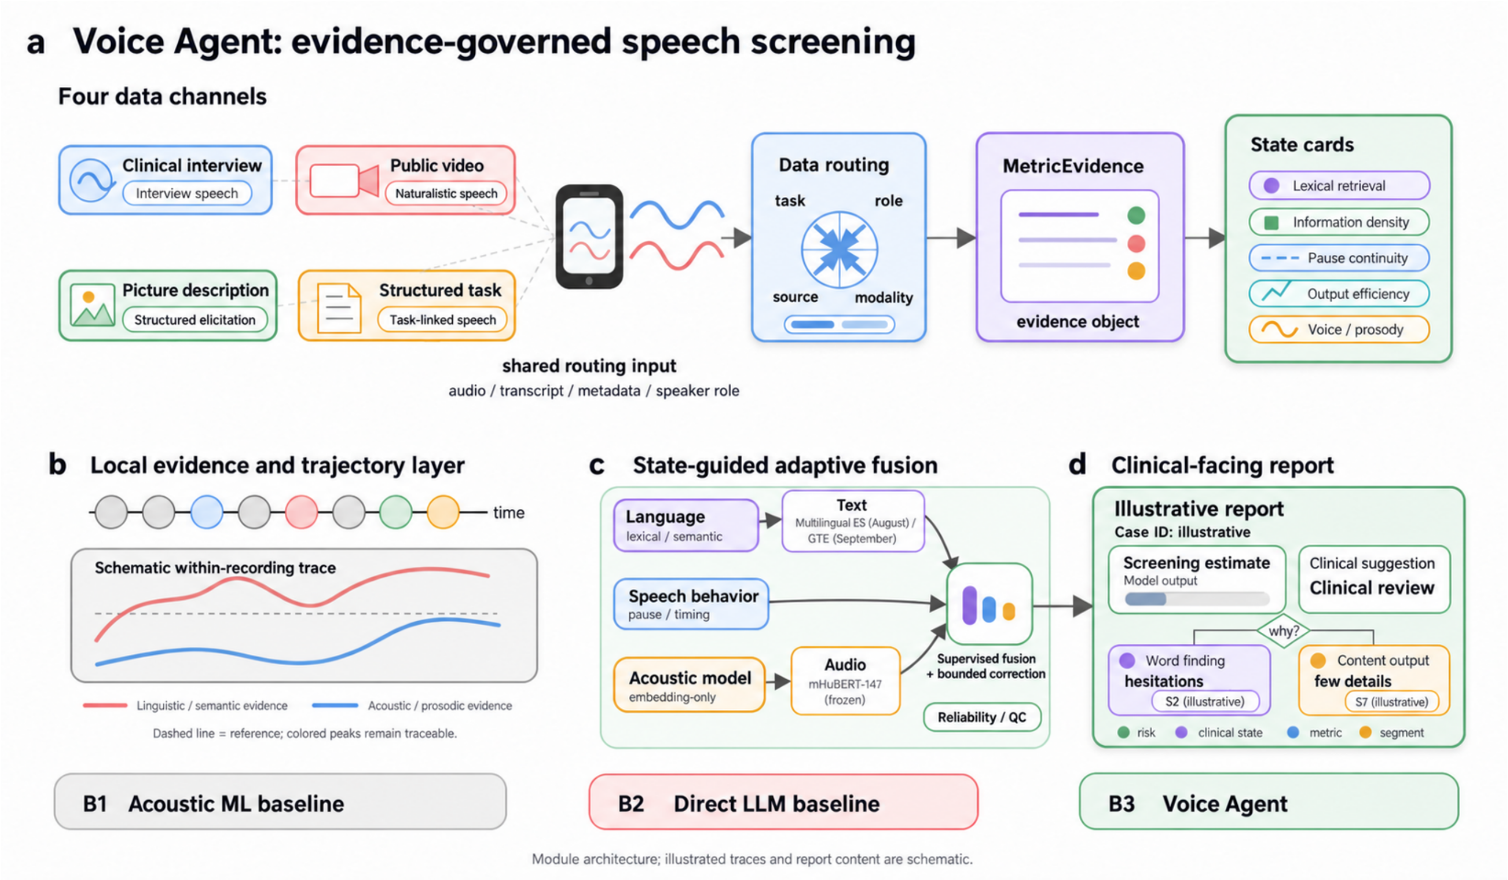
\includegraphics[width=\textwidth]{figures/2026-09-24_revision/Fig1_system_architecture.png}
\caption{Evidence-governed speech screening architecture. Audio, transcript, task metadata, speaker roles and optional model-only age context are routed into MetricEvidence objects and task-conditioned cognitive StateCards. Supervised experts estimate a calibrated risk, after which a constrained diagnostic Agent reviews only permitted evidence and produces a report tied to the locked decision.}
\label{fig:architecture}
\end{figure*}

\begin{figure*}[t]
\centering
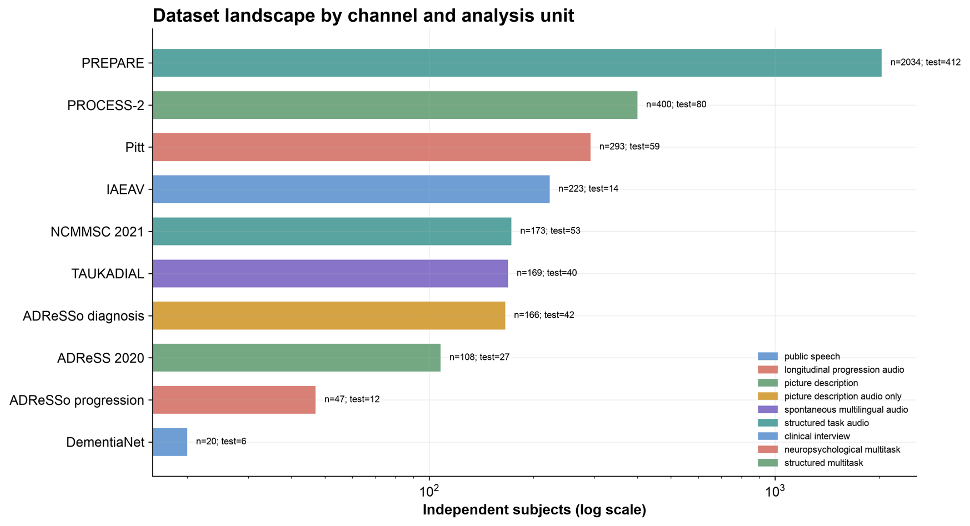
\includegraphics[width=\textwidth]{figures/2026-09-24_revision/Fig2_dataset_landscape.png}
\caption{Dataset landscape by data channel, language and source diagnostic target. Sector sizes reflect available analysis units rather than the 745 held-out units used for the matched three-condition evaluation. The figure motivates task- and source-specific routing and should not be interpreted as a pooled clinical cohort.}
\label{fig:landscape}
\end{figure*}

\subsection{Evidence-state fusion improved discrimination in most but not all tasks}

Ours had the highest macro-AUROC among the three conditions in seven of ten datasets (Table~\ref{tab:datasets}; Fig.~\ref{fig:performance}). Relative to B1, macro-AUROC increased in eight datasets, was unchanged in DementiaNet and decreased in the ADReSSo progression task. Relative to B2, it increased in seven datasets and decreased in progression, DementiaNet and TAUKADIAL. These counts are descriptive because the datasets differ in sample size, labels and task protocol; no simple pooled AUROC was treated as a universal performance estimate.

The clearest gains occurred on ADReSS 2020 (macro-AUROC 0.978, 95\% bootstrap confidence interval 0.919--1.000), ADReSSo diagnosis (0.857, 0.729--0.948), PROCESS-2 (0.862, 0.797--0.920) and PREPARE (0.811, 0.779--0.842). Corresponding held-out accuracies were 0.852, 0.810, 0.700 and 0.677. In contrast, Ours produced macro-AUROC 0.556 in ADReSSo progression and 0.516 in TAUKADIAL. DementiaNet macro-AUROC was 0.500 with a 0--1 bootstrap interval, demonstrating that the six-person evaluation is uninformative for comparative performance.

Calibration generally improved relative to the direct language-model condition. Ours had lower expected calibration error than B2 in nine of ten datasets and lower error than B1 in eight. This did not imply uniform safety: ECE was 0.231 in the small progression task and 0.389 in DementiaNet. PREPARE ECE was 0.079 compared with 0.041 for B1, illustrating that improved discrimination did not automatically imply better calibration than every comparator.

\begin{figure*}[t]
\centering
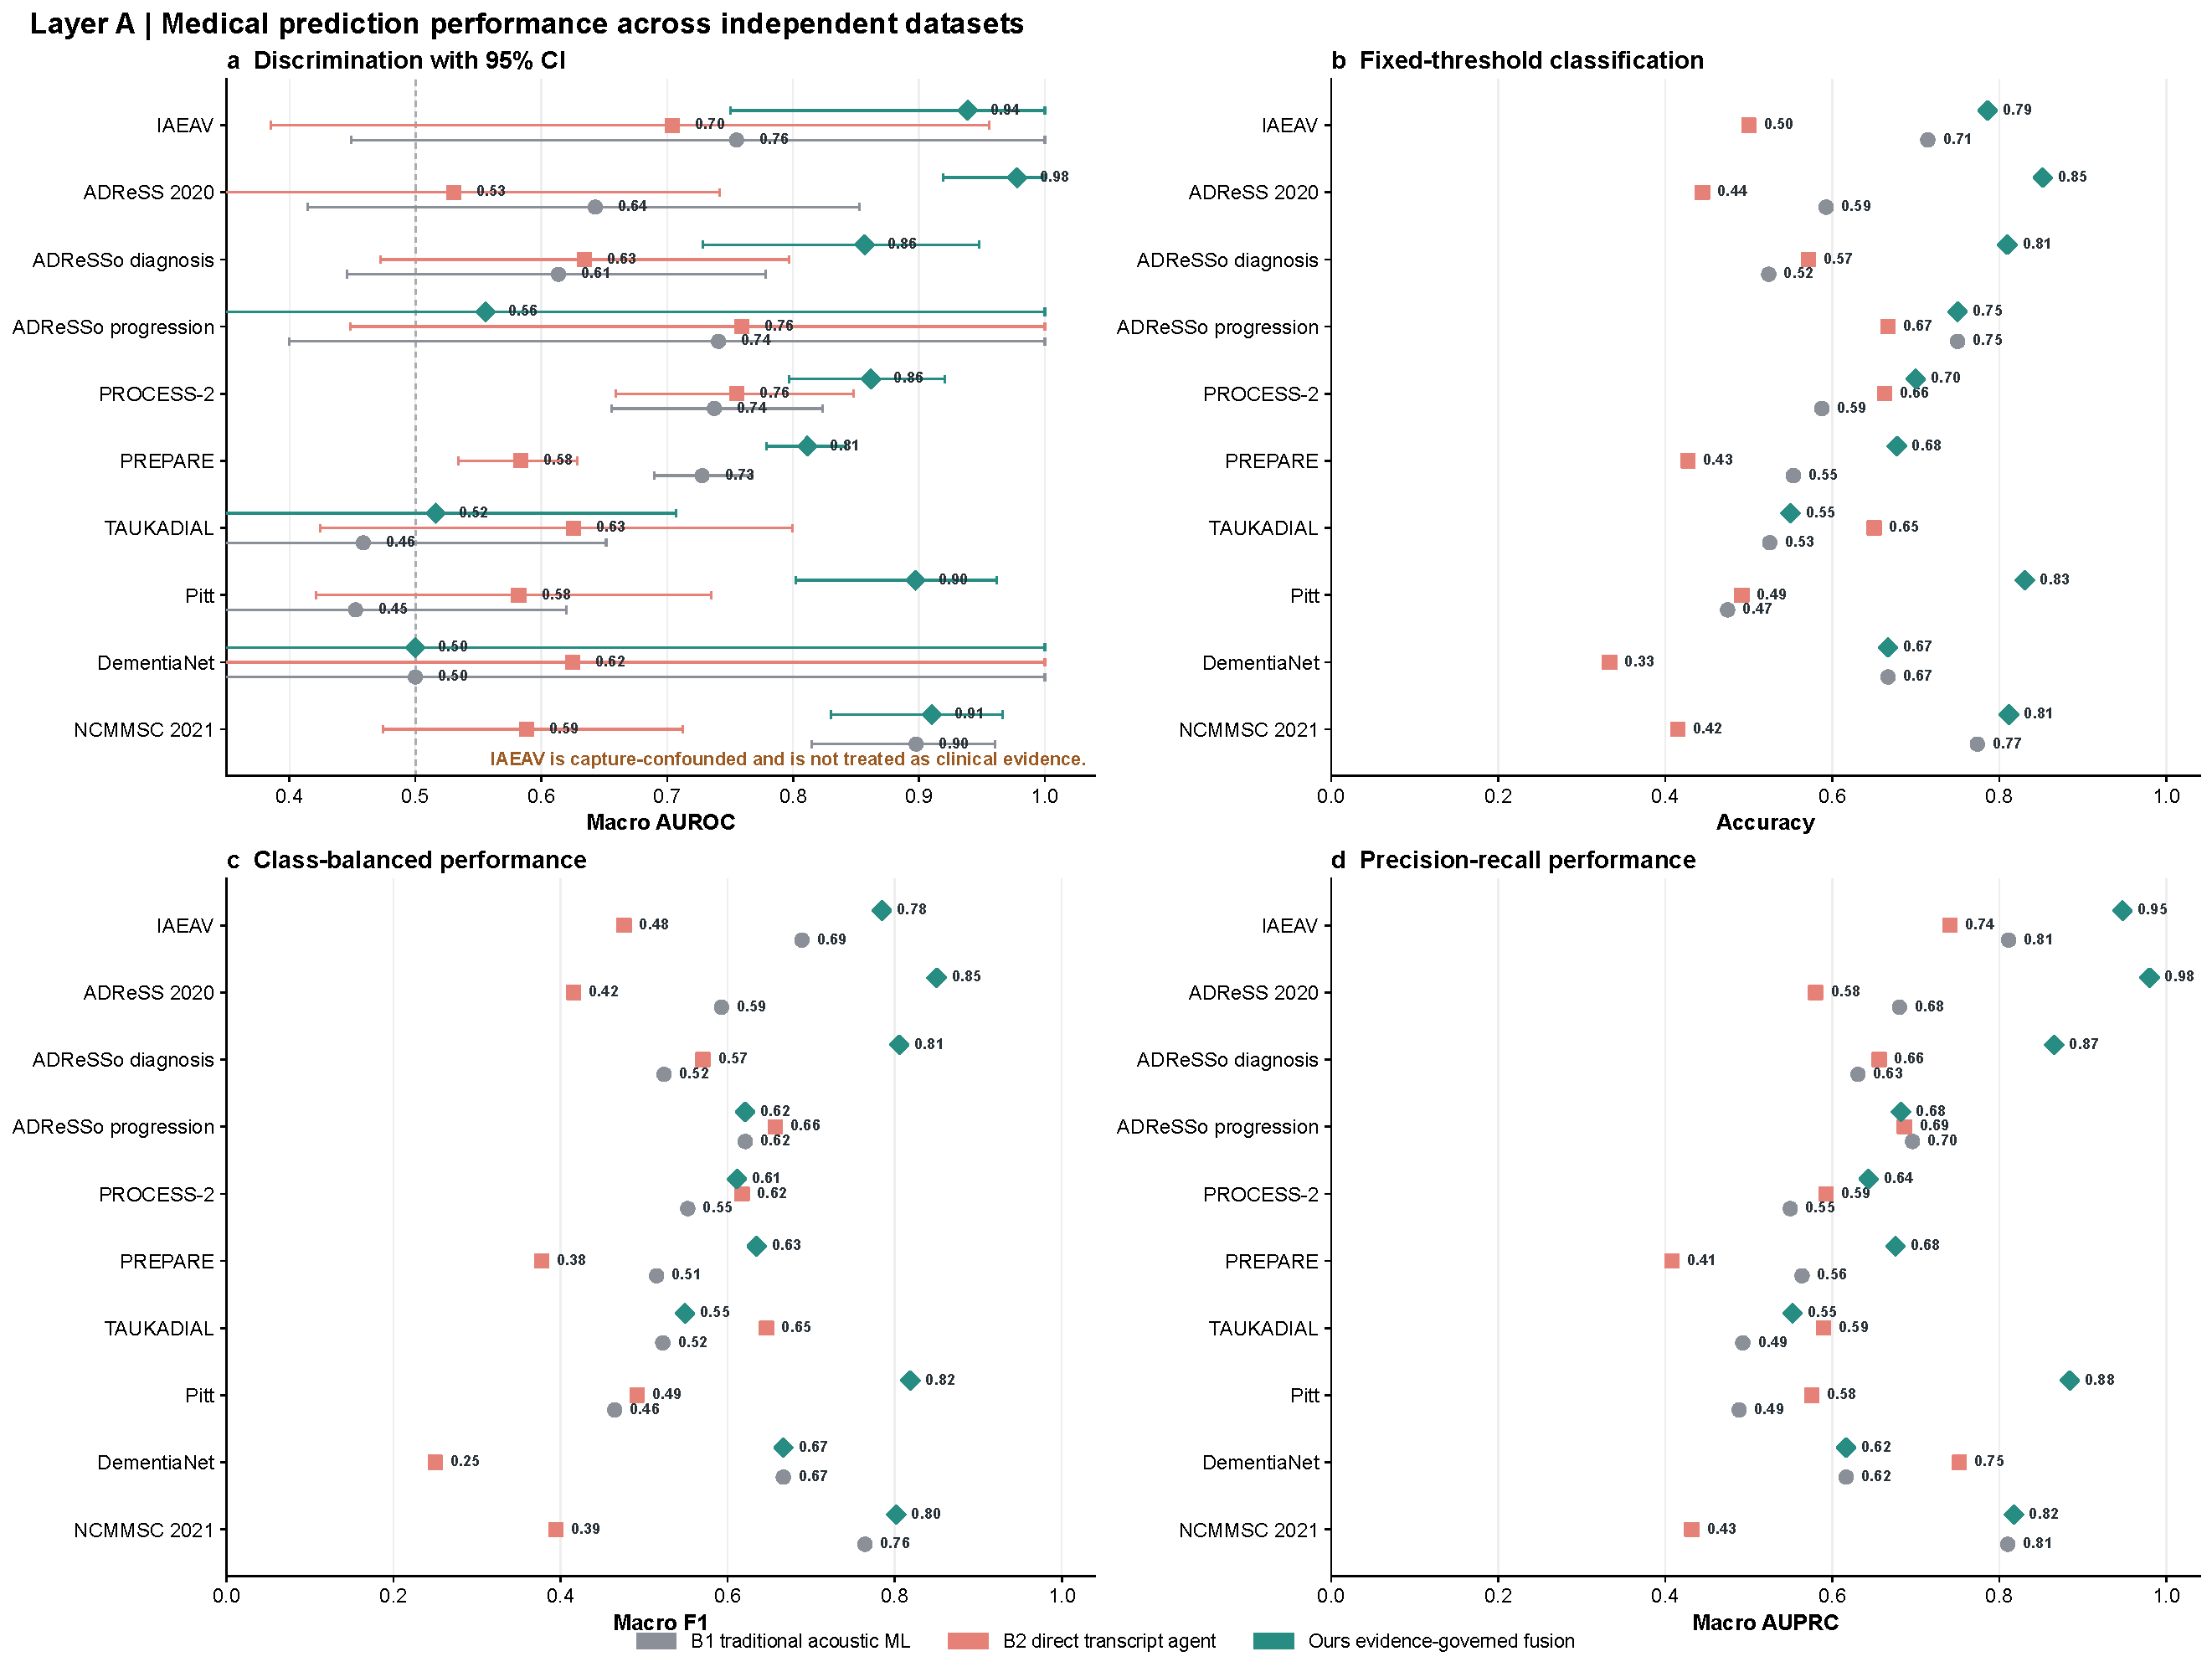
\includegraphics[width=\textwidth]{figures/latex_ready_new_figures_2026-08-27/main_figures/Fig3_predictive_performance.pdf}
\caption{Layer A predictive evaluation across matched held-out participants. Points and intervals show dataset-specific discrimination and classification performance for B1, B2 and Ours. Results should be interpreted with the cohort-specific bias flags rather than as a pooled leaderboard.}
\label{fig:performance}
\end{figure*}

\subsection{The PREPARE result remained below SpeechCARE}

PREPARE provided the closest dataset-level comparison with SpeechCARE. On the official test set, Ours achieved micro-AUROC 0.8325, micro-F1/accuracy 0.6772, weighted AUROC 0.7852, micro-AUPRC 0.6797 and weighted AUPRC 0.7152. SpeechCARE reported 0.8683, 0.7211, 0.8067, 0.7473 and 0.7350, respectively \cite{Azadmaleki2025}. The differences were therefore $-0.0358$, $-0.0439$, $-0.0215$, $-0.0676$ and $-0.0198$. SpeechCARE reports the mean of ten training runs, whereas the present evaluation used a locked run with participant bootstrap uncertainty. We consequently treat this as a protocol-aware descriptive comparison, not evidence that either architecture is statistically superior under identical repeated training.

\subsection{Quality controls exposed dataset shortcuts}

Negative controls were used to test whether recording or task structure alone separated labels. IAEAV was downgraded because interviewer/acquisition groups were strongly aligned with diagnostic labels. In DementiaBank Pitt, a quality-control-only model reached macro-AUROC 0.788 despite the complete model reaching 0.897. In NCMMSC, the corresponding values were 0.832 and 0.910. These results indicate that high discrimination can coexist with substantial non-cognitive signal. The framework prevented quality variables from being written as disease mechanisms, but residualization and report permissions do not by themselves establish that the predictive model is free of dataset shortcuts. We therefore exclude these three results from the strongest clinical-validity claim.

\begin{figure*}[t]
\centering
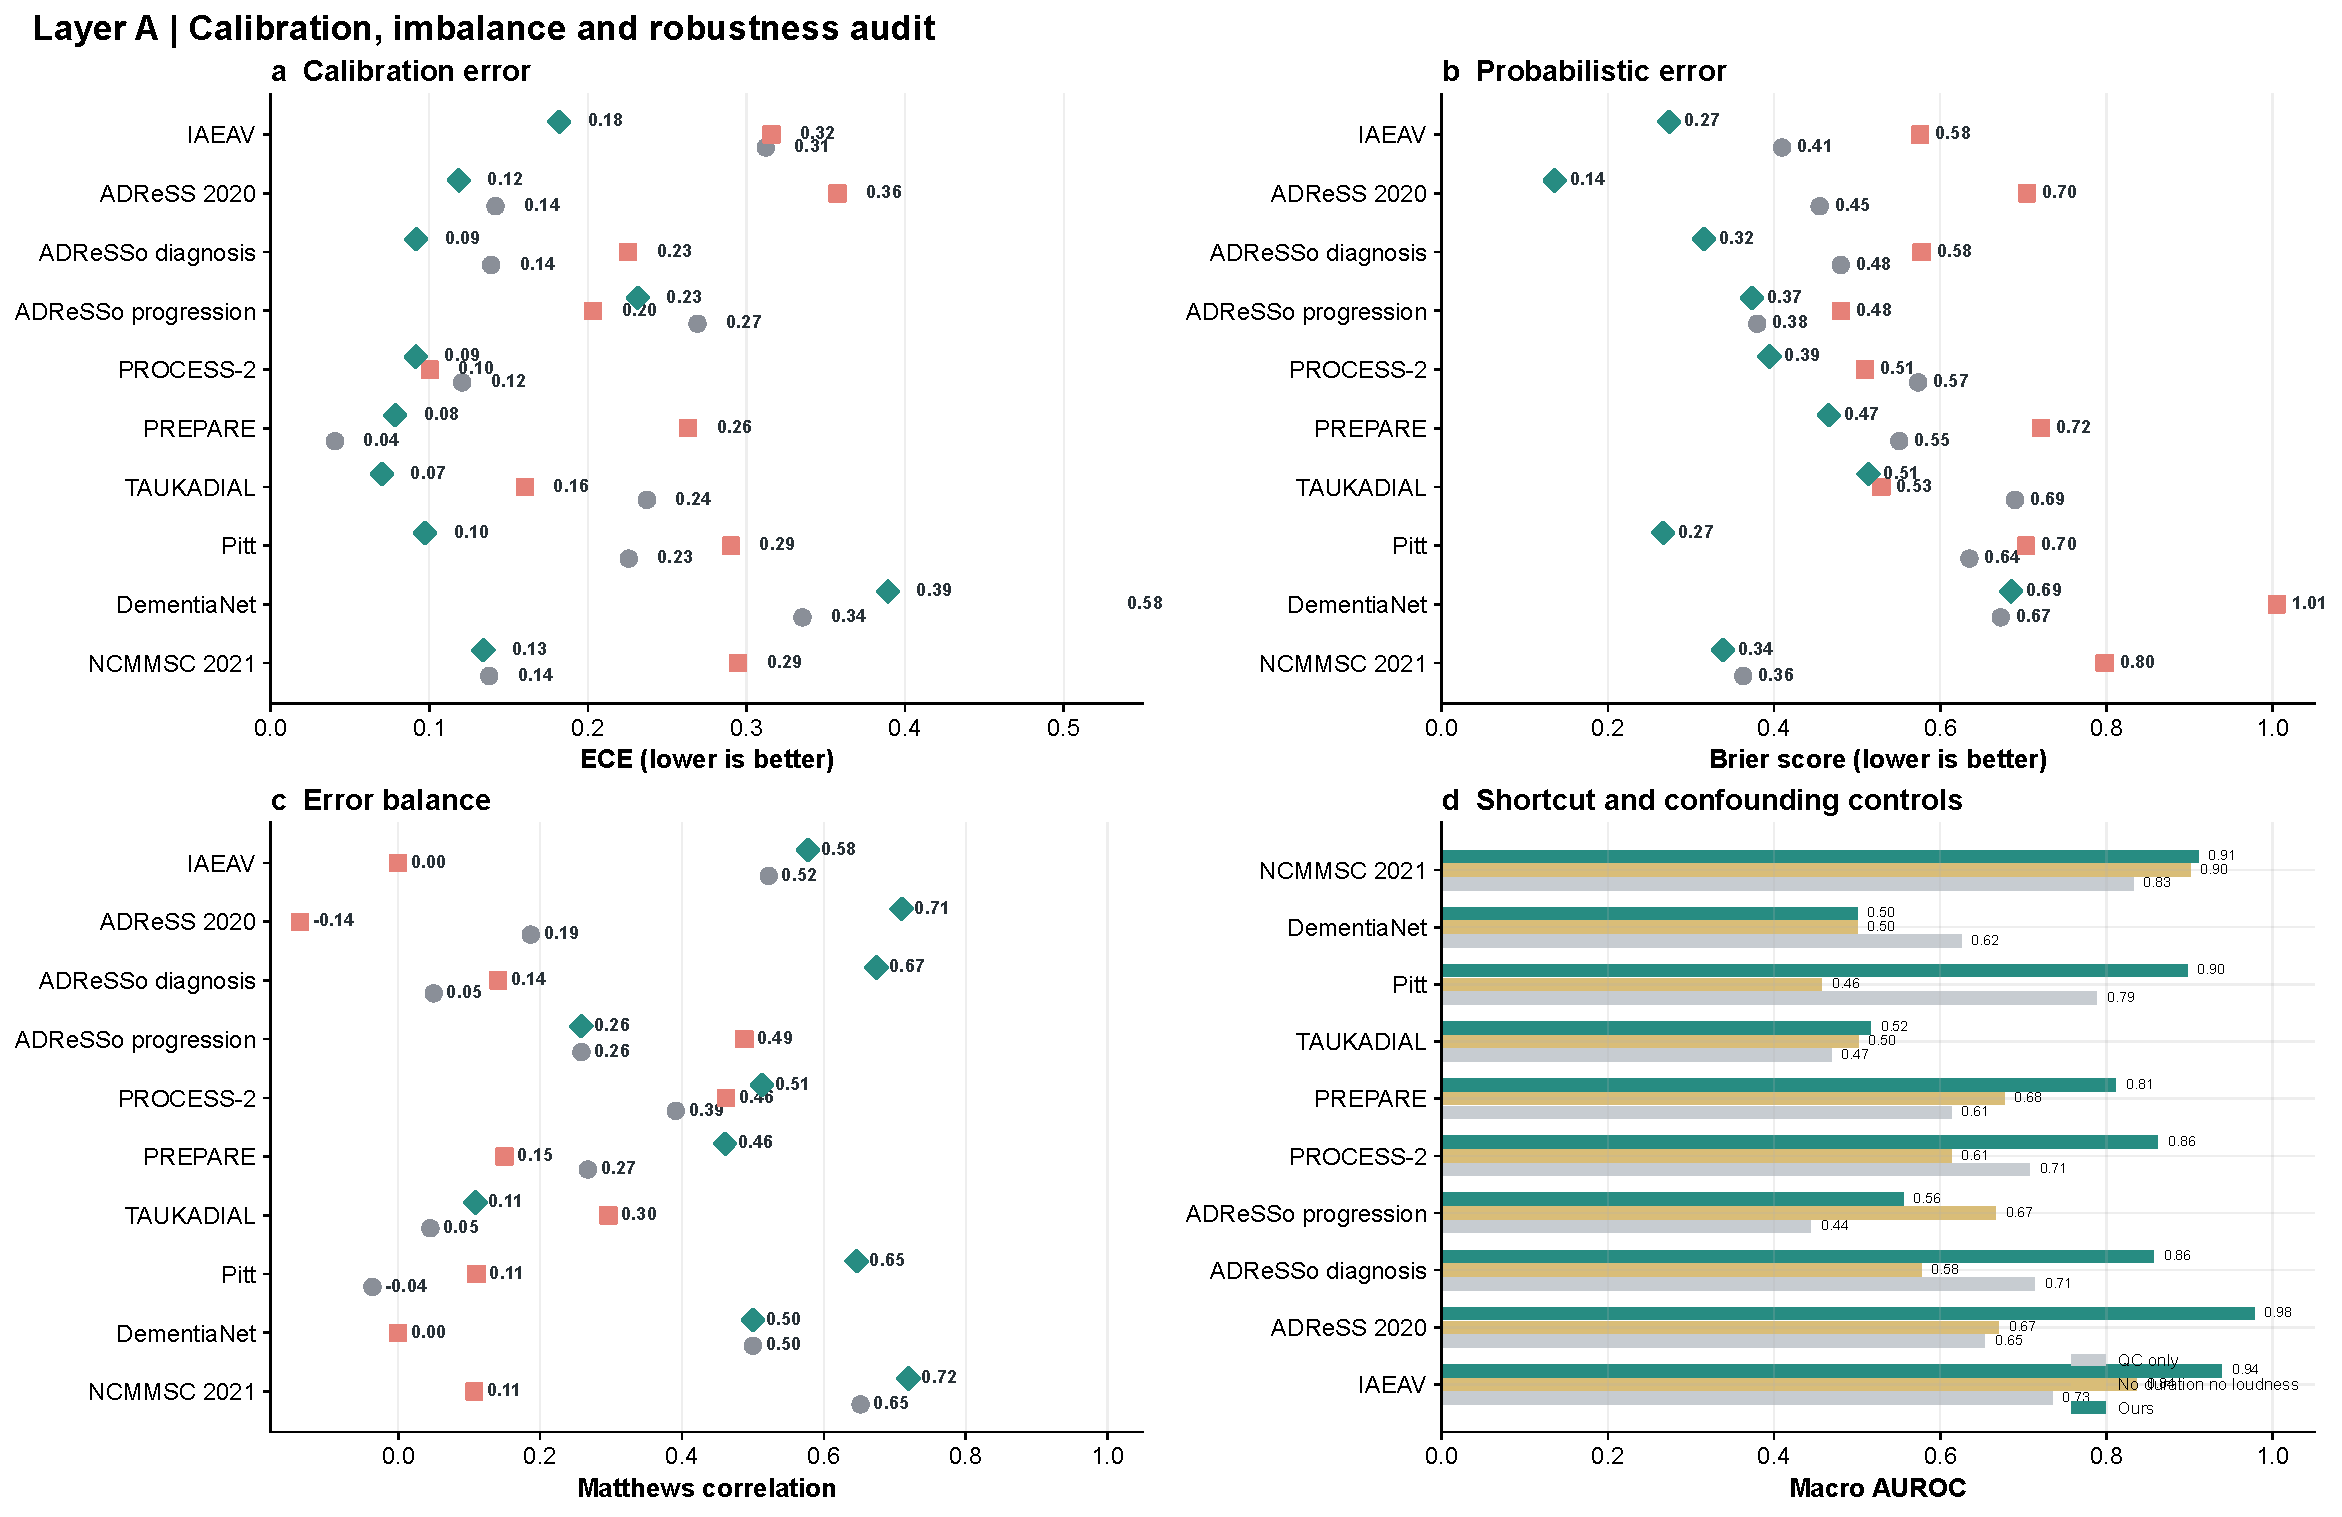
\includegraphics[width=\textwidth]{figures/latex_ready_new_figures_2026-08-27/main_figures/Fig4_calibration_safety.pdf}
\caption{Calibration, screening and shortcut audit. The panels summarize expected calibration error, threshold behaviour, high-confidence error and quality-control negative controls. Lower calibration and error measures are preferable, whereas a high quality-control-only AUROC indicates potential acquisition bias.}
\label{fig:safety}
\end{figure*}

\subsection{The evidence chain was complete but Agent proposals were often invalid}

MetricEvidence and StateCard schema completeness was 1.00 in all ten datasets, and every locally traceable speech-behaviour citation resolved to the same case, source interval and state-specific selection rule. Branch contributions were finite and normalized, and report-permission audits prevented quality-control and low-interpretability model features from appearing as disease-supporting clinical evidence. These checks demonstrate implementation consistency, not clinical validity of every state definition.

The diagnostic Agent returned a structured candidate for every preregistered held-out case, but candidate evidence validity averaged 0.509 across datasets (range 0.288--1.000). Invalid or unsupported candidates were rejected. No bounded Agent correction was applied, no class decision changed, and Agent-on versus Agent-off differences in macro-AUROC and accuracy were zero. Thus, the predictive gains reported above arose from supervised evidence-state fusion and calibration, not from language-model correction. The safe-fallback report template was invoked for a mean 38.3\% of audited cases, including every audited PROCESS-2 report, identifying report validation as an unresolved engineering limitation.

Automated, blinded report-structure scoring across five dimensions gave a dataset-level mean of 20.66/25 for Ours and 11.66/25 for B2 (Figs.~\ref{fig:framework} and~\ref{fig:reports}). The dimensions were evidence completeness, clinical interpretability, safety/calibration, screening usefulness and traceability. Because the evaluator was an automated model rather than a clinician, this result supports structural compliance only and cannot establish clinical usefulness or physician acceptance.

\begin{figure*}[t]
\centering
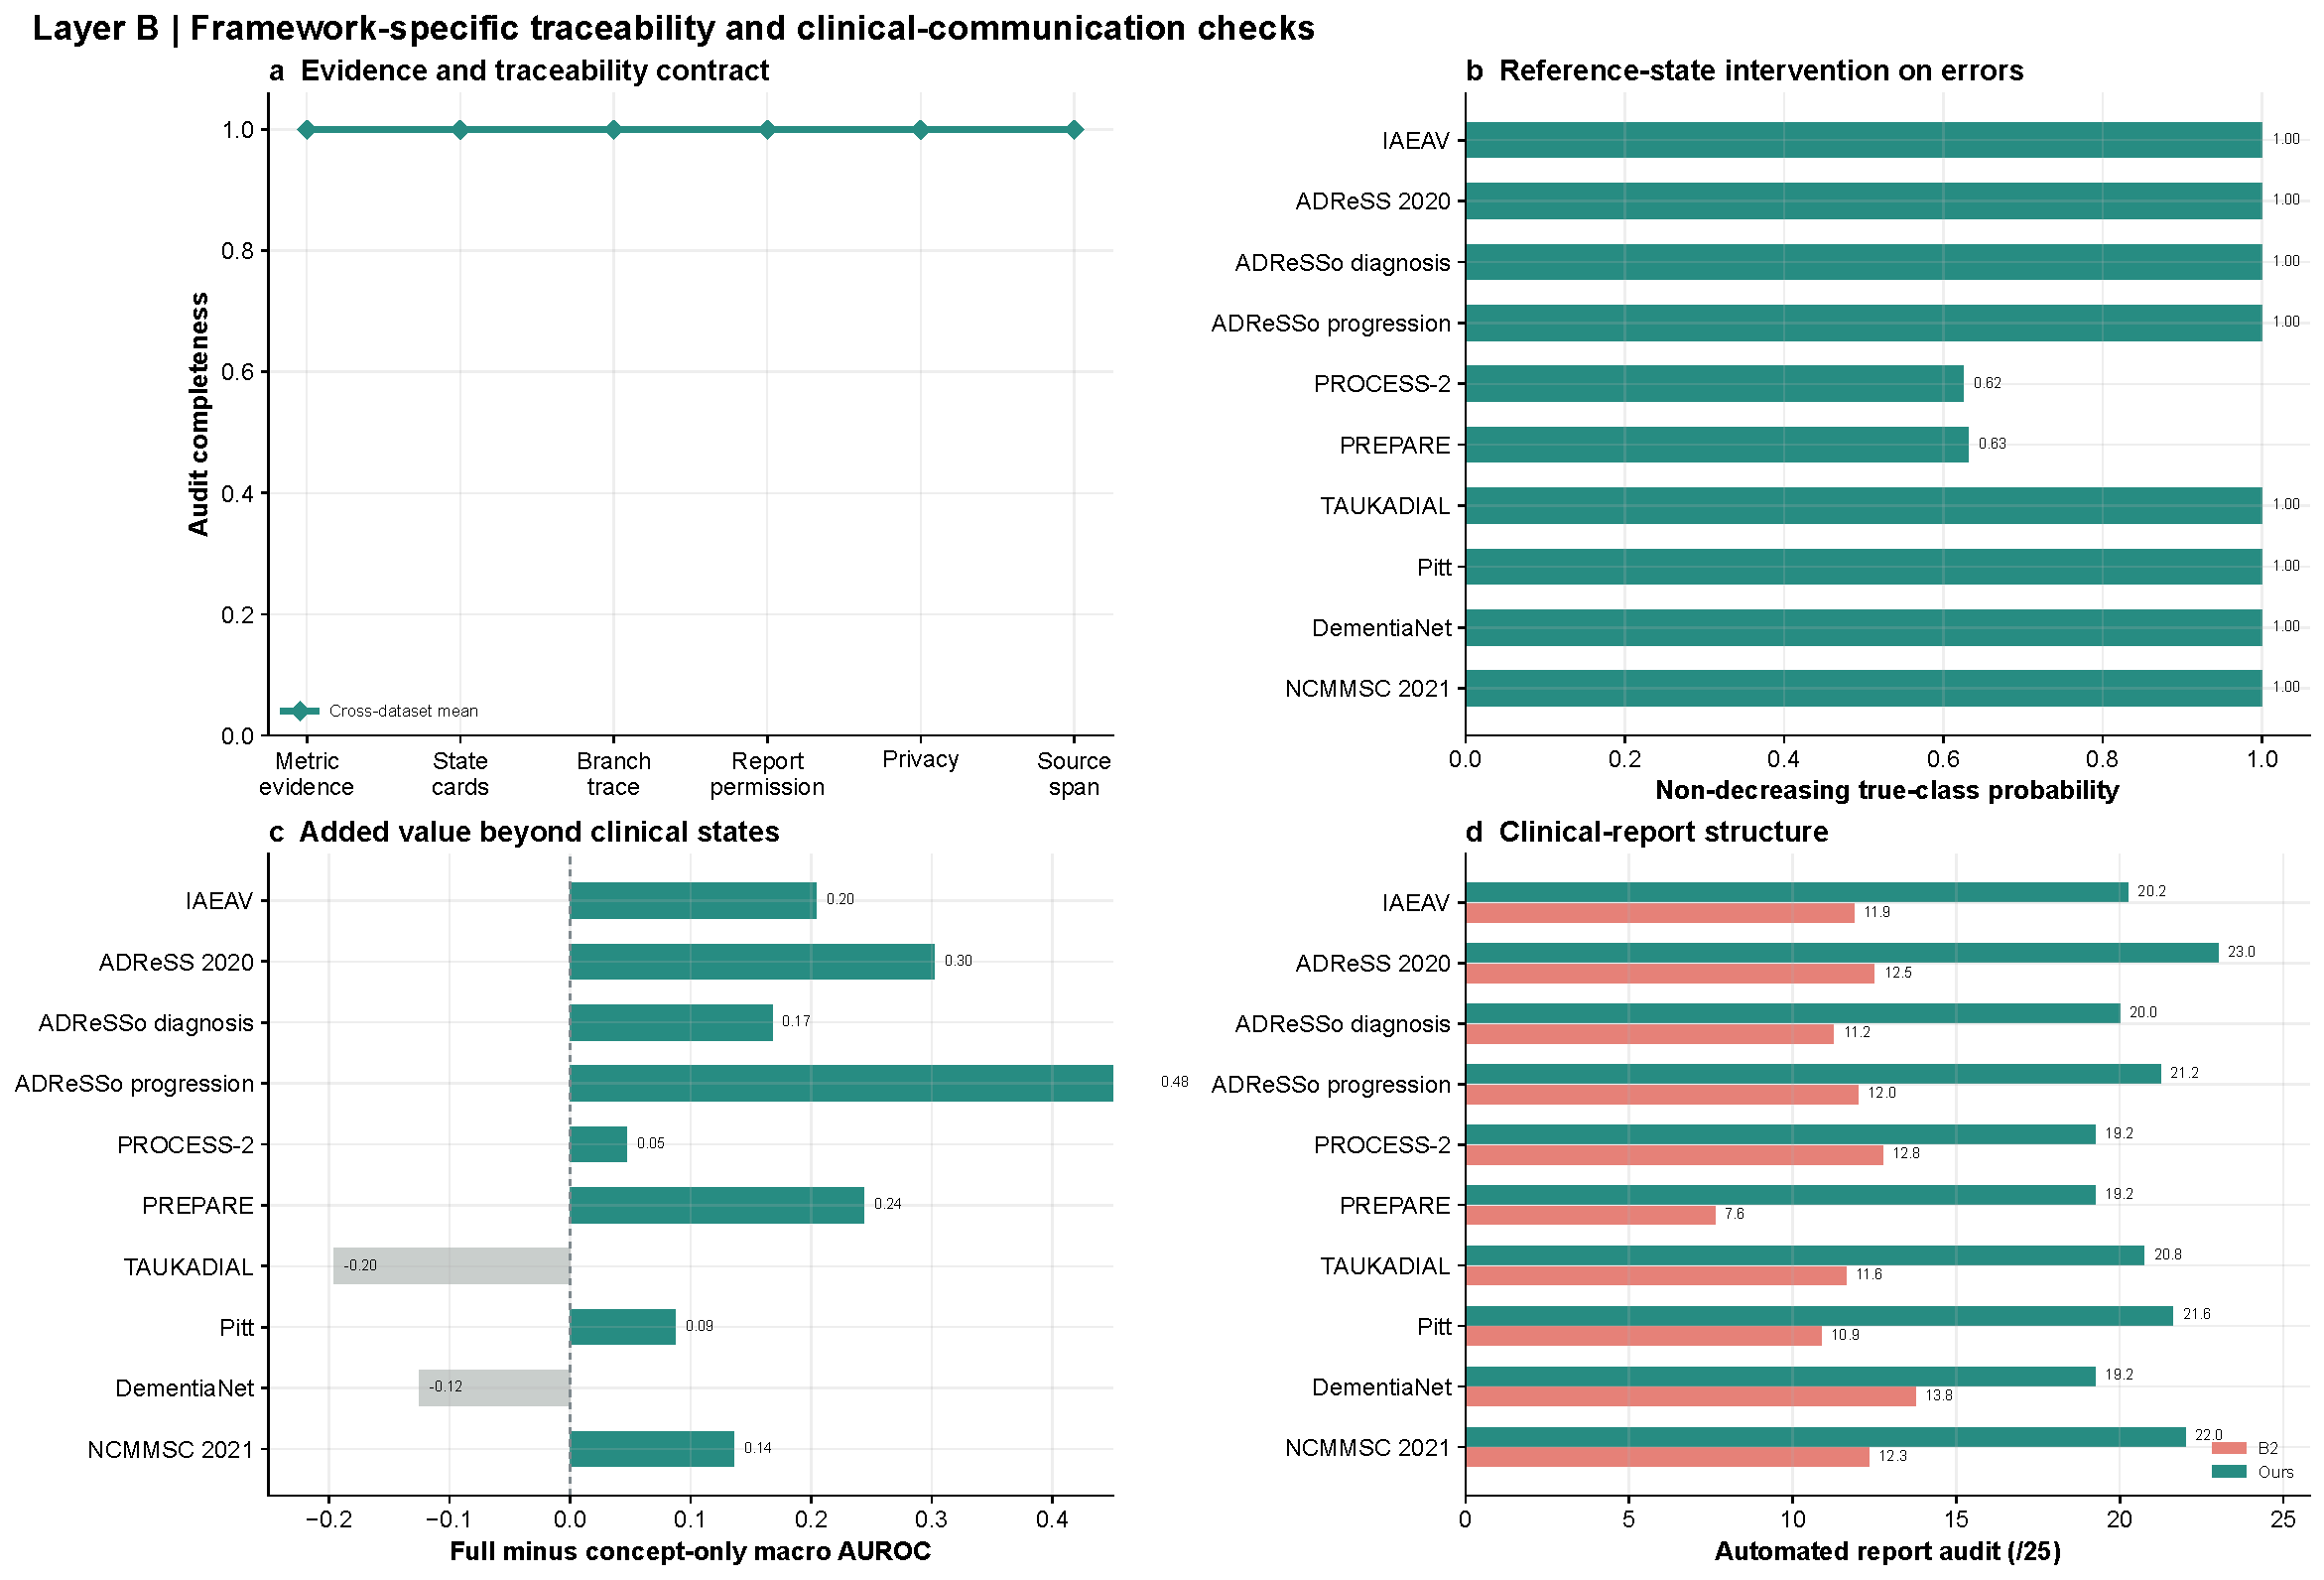
\includegraphics[width=\textwidth]{figures/latex_ready_new_figures_2026-08-27/main_figures/Fig5_framework_validation.pdf}
\caption{Layer B framework validation. Checks quantify evidence-object completeness, cognitive-state completeness, branch traceability, report permissions, segment faithfulness, intervention consistency and automated report structure. These measures test whether the claimed evidence pathway exists; they do not replace physician evaluation.}
\label{fig:framework}
\end{figure*}

\begin{figure*}[t]
\centering
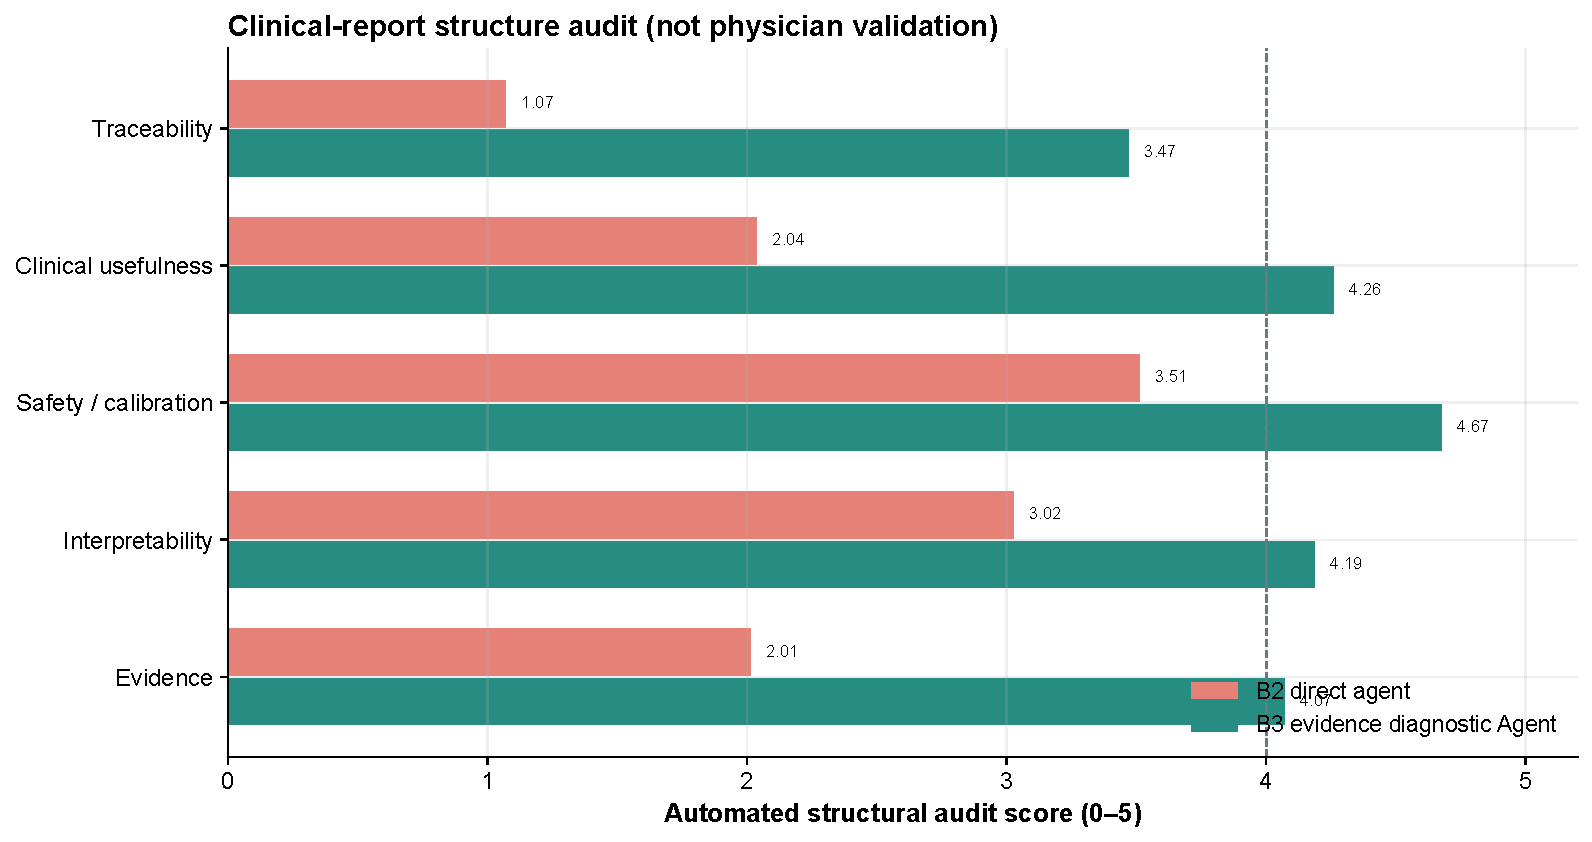
\includegraphics[width=\textwidth]{figures/latex_ready_new_figures_2026-08-27/main_figures/Fig6_report_rubric.pdf}
\caption{Automated report-structure comparison between the direct language-model condition and Ours. The five-domain rubric evaluates evidence completeness, clinical interpretability, safety and calibration language, screening usefulness and traceability. Scores are produced by an automated evaluator and are not physician ratings.}
\label{fig:reports}
\end{figure*}

\begin{figure*}[t]
\centering
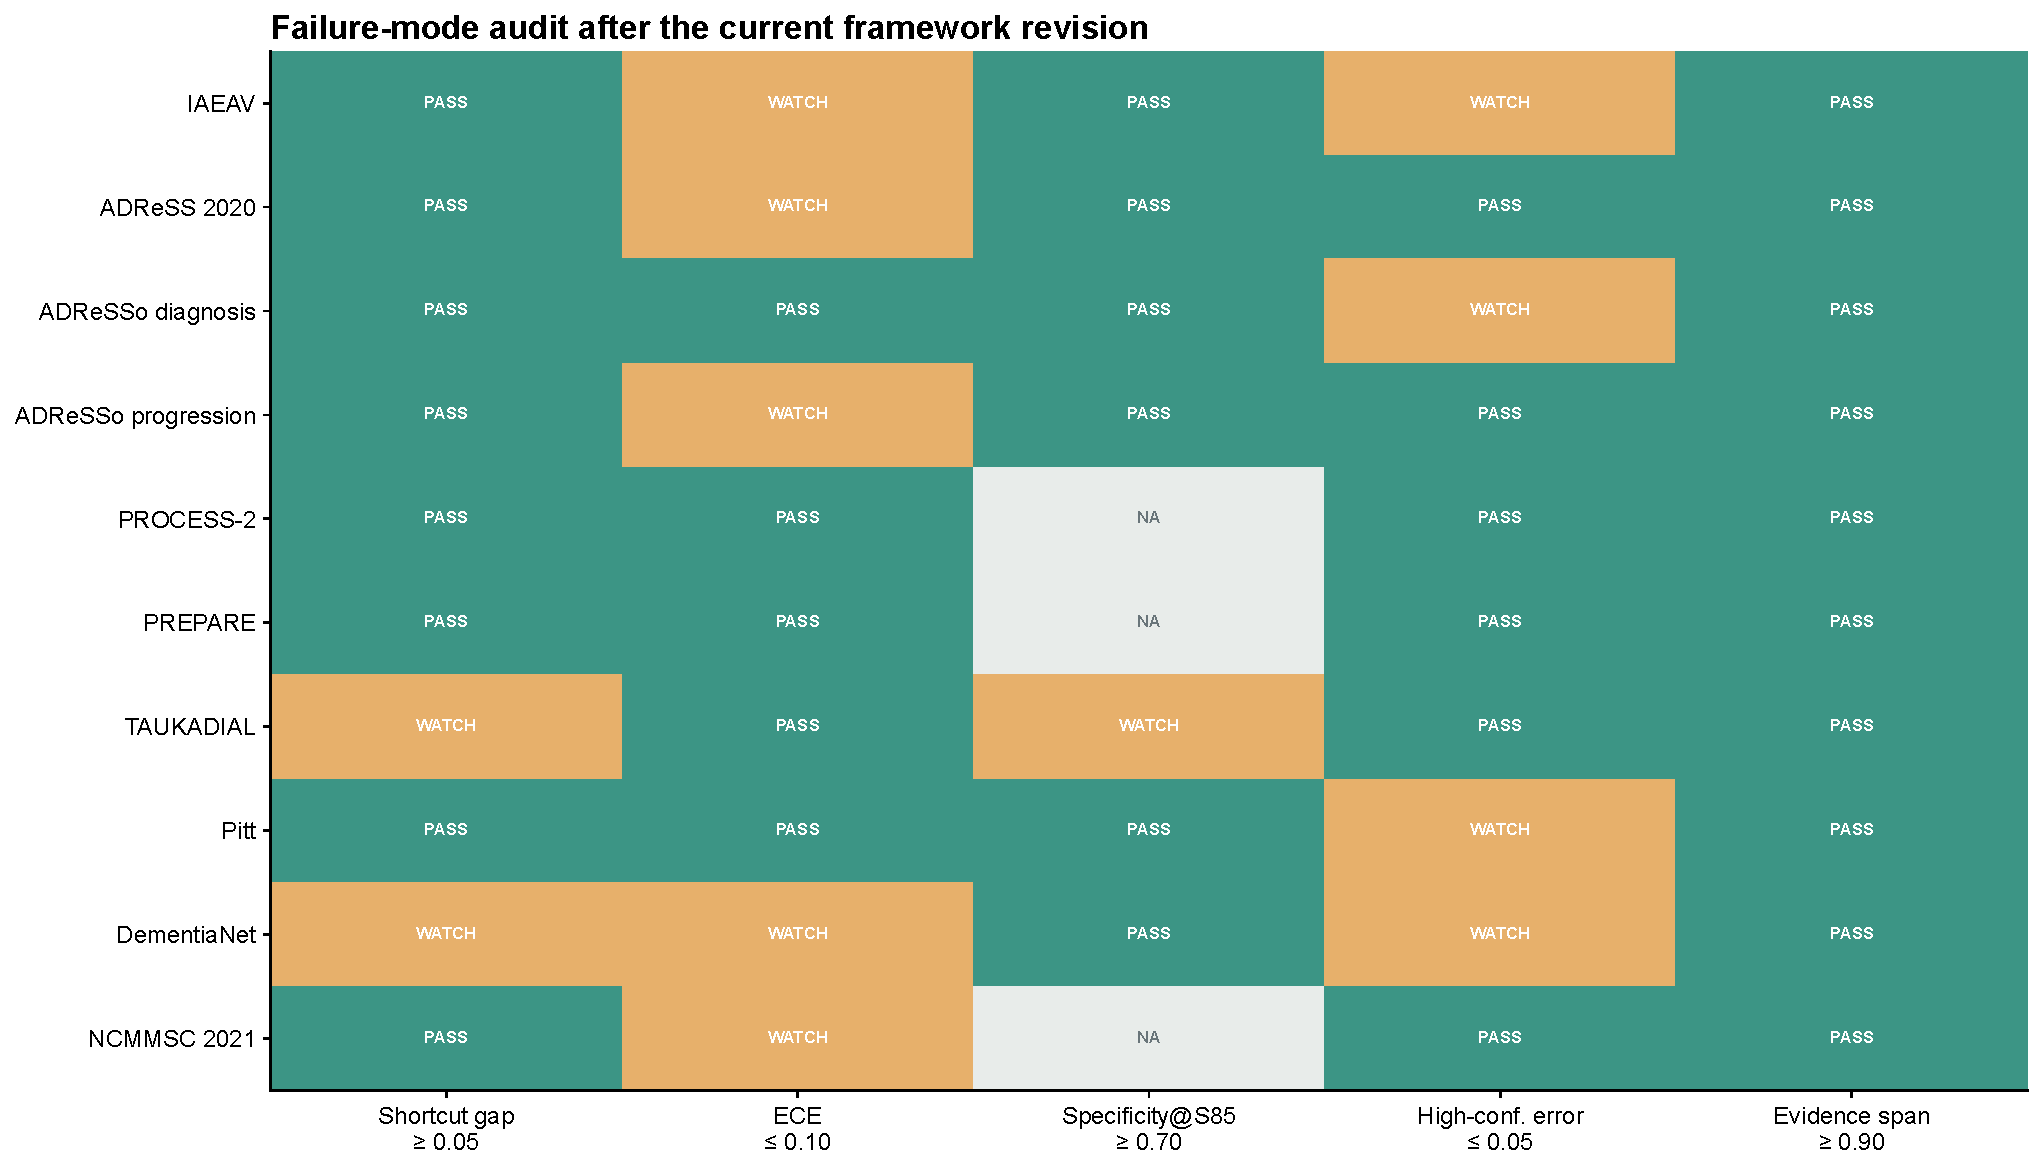
\includegraphics[width=\textwidth]{figures/latex_ready_new_figures_2026-08-27/main_figures/Fig7_failure_modes.pdf}
\caption{Failure-mode audit after the locked evaluation. Progression, cross-language spontaneous speech, acquisition confounding, quality-control shortcuts and invalid Agent evidence candidates define the current limits of the framework. Repairs shown in the figure are engineering safeguards or planned validation steps and should not be interpreted as completed clinical validation.}
\label{fig:failures}
\end{figure*}

\section{Discussion}\label{sec:discussion}

This study suggests that a cognitive-state layer can provide a useful intermediate interface between heterogeneous speech tasks and clinical screening outputs. Rather than forcing picture description, interview, structured task and spontaneous speech into a single undifferentiated feature vector, the framework first determines which states are observable in each task and how reliable each measurement is for the current case. This organization improved discrimination over conventional acoustic machine learning and a direct language model in most evaluated tasks, while retaining a trace from the final report to the task, state, metric and local source segment.

The contribution differs from SpeechCARE's adaptive modality fusion. SpeechCARE learns how strongly a sample should rely on acoustic, linguistic and demographic representations and currently performs better on PREPARE \cite{Azadmaleki2025}. Our framework instead constrains what those representations are allowed to mean clinically. Modality-level gating and cognitive-state evidence are complementary: the former is optimized for predictive representation, whereas the latter specifies task observability, patient-level reliability, confounding and report permission. The present results do not show that interpretability compensates for lower predictive performance. A direct, repeated-seed PREPARE comparison and stronger multilingual encoders are required before performance equivalence with SpeechCARE can be claimed.

The contribution also differs from MEDRF. MEDRF uses clinical profiles and structural MRI to predict a diagnostic hierarchy, then retrieves analogous cases and literature to refine ambiguous predictions \cite{Hu2026}. Our hierarchy is a measurement pathway rather than a diagnostic ontology: local speech segments support metrics, metrics support cognitive states, and states support a screening probability. This design is intended for settings without imaging or complete neuropsychological profiles. However, MEDRF demonstrated actual prediction gains from RAG-LLM correction and obtained physician evaluations, whereas our Agent changed no probabilities and our report score was automated. The current evidence therefore supports an evidence-governed reporting and safety layer, not an autonomous diagnostic Agent.

The failure analyses are as important as the favourable datasets (Fig.~\ref{fig:failures}). Progression prediction did not benefit from the cross-sectional state architecture, suggesting that longitudinal change requires within-person baselines and trajectory-specific supervision. TAUKADIAL exposed weak transfer to Mandarin--English spontaneous speech, where ASR, language-specific lexical measurement and label definition differ from structured picture description. IAEAV, Pitt and NCMMSC showed that acquisition and quality variables can be highly predictive. Preventing these variables from appearing in the report is necessary, but it does not prevent correlated latent representations from exploiting them. Future evaluation should therefore use leave-site, leave-task and leave-language protocols, adversarial dataset-identity tests and prospective collection with balanced devices and interviewers.

Several limitations constrain clinical interpretation. This was a retrospective benchmark assembled from datasets with different labels and reference standards; it was not a prospective screening trial. The 745 held-out units should not be treated as one exchangeable clinical cohort. Some confidence intervals were wide, particularly for progression, IAEAV and DementiaNet. State definitions were literature-informed but have not yet undergone formal clinician content-validity assessment. The report evaluator was automated, and no blinded clinician comparison measured decision quality, review time or referral appropriateness. The Agent evidence validator rejected many candidates and applied no risk corrections. Finally, the framework predicts dataset labels for research screening; it cannot determine Alzheimer pathology, distinguish all alternative causes of cognitive impairment or recommend treatment.

Within these boundaries, the results establish a reproducible separation between predictive evidence, quality control and clinical communication. A clinically useful next version should combine SpeechCARE-level multilingual representation learning with the present state and provenance constraints, then evaluate whether clinicians can correct a state, observe a coherent probability change and make better referral decisions. That experiment, rather than another increase in automatically generated report fluency, would test whether the evidence chain improves care.

\section*{Data availability}

The study used datasets distributed under their respective source agreements. Several source recordings cannot be redistributed by the authors. Dataset adapters, inclusion rules, pseudonymous split identifiers and derived aggregate statistics will be released subject to those agreements. \textbf{[AUTHOR INPUT REQUIRED: list accession links, approval identifiers and the exact derived data that can be shared.]}

\section*{Code availability}

The complete analysis code, configuration files, tests and report-generation workflow are maintained in the 8.27 project repository. \textbf{[AUTHOR INPUT REQUIRED: provide a public repository URL, immutable release tag, license and archival DOI before submission.]}

\backmatter

\bmhead{Acknowledgements}
\textbf{[AUTHOR INPUT REQUIRED: funding, computing support and contributors.]}

\bmhead{Author contributions}
\textbf{[AUTHOR INPUT REQUIRED: CRediT contributions using author initials.]}

\bmhead{Competing interests}
The authors declare no competing interests.

\bmhead{Ethics declaration}
\textbf{[AUTHOR INPUT REQUIRED: secondary-data ethics determination, original cohort approvals and consent statements.]}

\bibliography{references}

\end{document}
